\chapter{Infrastructure PKI et HashiCorp Vault}

\section{Conception de la hiérarchie de certification}

\subsection{Principes de conception}

L'infrastructure PKI adoptée suit une hiérarchie à \textbf{deux niveaux} : une CA racine et une CA intermédiaire. Ce schéma est recommandé par le NIST (SP~800-57)~\cite{nist_sp800213} pour plusieurs raisons :

\begin{itemize}
  \item La CA racine peut rester hors-ligne (\textit{offline CA}), réduisant sa surface d'attaque.
  \item La CA intermédiaire, exposée aux systèmes applicatifs, peut être révoquée et remplacée sans invalider toute la chaîne.
  \item Les politiques de certification (contraintes de nommage, durées de vie) sont définies indépendamment par niveau.
\end{itemize}

La figure~\ref{fig:pki_hierarchy} présente le diagramme de classes de la hiérarchie PKI, montrant les relations entre la CA racine, la CA intermédiaire, les rôles d'émission et les certificats de dispositifs.

\begin{figure}[H]
  \centering
  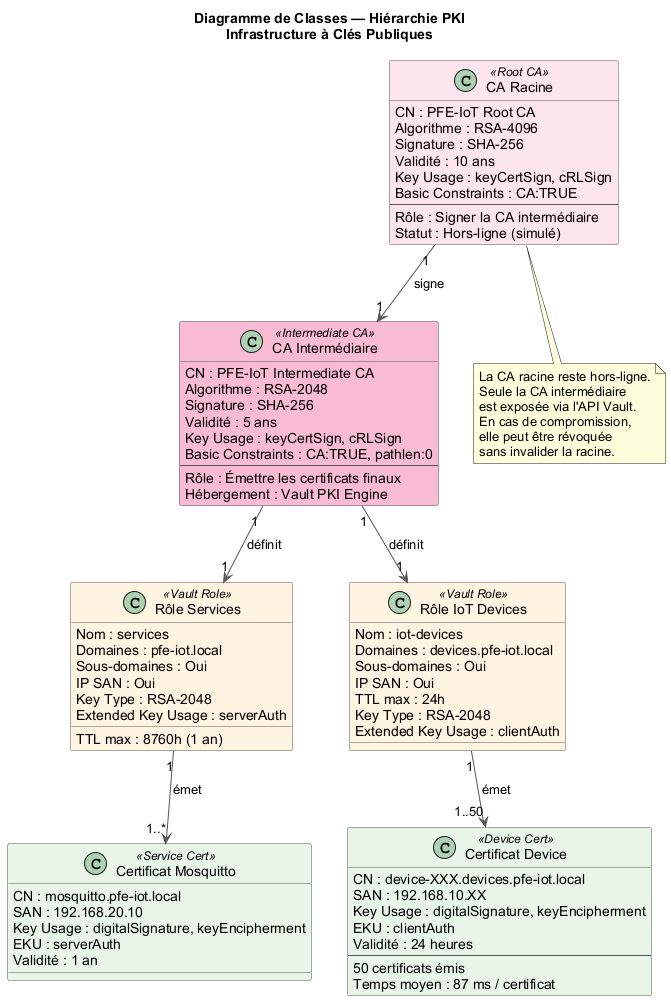
\includegraphics[width=0.8\textwidth]{diagrams/diag-pki-hierarchy.png}
  \caption{Hiérarchie PKI -- diagramme de classes}
  \label{fig:pki_hierarchy}
\end{figure}

\subsection{Paramètres cryptographiques}

\begin{table}[H]
\centering
\caption{Paramètres cryptographiques de la PKI}
\label{tab:pki_params}
\begin{tabular}{lll}
\toprule
\textbf{Paramètre} & \textbf{CA Racine} & \textbf{CA Intermédiaire} \\
\midrule
Algorithme de clé & RSA-4096 & RSA-2048 \\
Algorithme de signature & SHA-256 & SHA-256 \\
Durée de validité & 10 ans & 5 ans \\
Profil de certificat & CA basic constraint & CA basic constraint \\
\bottomrule
\end{tabular}
\end{table}

Pour les certificats \textbf{dispositifs et services}, les paramètres retenus sont :
\begin{itemize}
  \item \textbf{Algorithme} : RSA-2048 / SHA-256.
  \item \textbf{Validité} : 24~heures (dispositifs IoT -- renouvellement automatique via script).
  \item \textbf{SAN (Subject Alternative Name)} : Inclut l'IP de la machine et le nom DNS.
  \item \textbf{Key Usage} : \texttt{digitalSignature, keyEncipherment}.
  \item \textbf{Extended Key Usage} : \texttt{clientAuth} (dispositifs), \texttt{serverAuth} (Mosquitto).
\end{itemize}

\section{Déploiement de HashiCorp Vault}

\subsection{Configuration initiale}

Vault est déployé dans un conteneur Docker basé sur l'image officielle \texttt{hashicorp/vault:1.15}~\cite{vault_pki}. Il est configuré en mode \textbf{development} pour ce prototype, avec un backend de stockage en mémoire. Pour un déploiement production, un backend Consul ou Raft (intégré) serait recommandé.

Le processus d'initialisation comprend les étapes suivantes :
\begin{enumerate}
  \item \textbf{Initialisation} du serveur Vault avec génération des clés de déverrouillage (\textit{unseal keys}) selon un schéma de Shamir (3 parts, seuil de 2).
  \item \textbf{Déverrouillage} (\textit{unseal}) du coffre-fort avec deux clés.
  \item \textbf{Authentification} avec le jeton racine (\textit{root token}).
  \item \textbf{Activation du moteur PKI} racine avec configuration du TTL maximal à 10~ans.
\end{enumerate}

L'intégralité des commandes d'initialisation est documentée dans le script \texttt{bootstrap-pki-api.sh} (voir Annexe~A, section~\ref{sec:script_pki}).

\subsection{Création de la CA racine}

La CA racine est générée en interne par Vault (mode \texttt{internal}) avec les paramètres suivants :
\begin{itemize}
  \item Common Name : \texttt{PFE-IoT Root CA}
  \item Type de clé : RSA-4096
  \item Durée de validité : 87\,600~heures (10 ans)
\end{itemize}

Le certificat racine est exporté sous forme de fichier PEM (\texttt{root-ca.crt}) pour être distribué aux clients comme ancre de confiance (\textit{trust anchor}).

\subsection{Création de la CA intermédiaire}

La CA intermédiaire est créée en trois étapes :
\begin{enumerate}
  \item \textbf{Génération du CSR} par le moteur \texttt{pki\_int} de Vault.
  \item \textbf{Signature du CSR} par la CA racine, produisant le certificat intermédiaire.
  \item \textbf{Import du certificat signé} dans le moteur \texttt{pki\_int}.
\end{enumerate}

Ce processus est entièrement automatisé via l'API REST de Vault (voir Annexe~A).

\subsection{Définition des rôles d'émission}

Deux rôles sont définis pour contrôler les types de certificats émissibles :

\begin{table}[H]
\centering
\caption{Rôles d'émission PKI définis dans Vault}
\label{tab:vault_roles}
\begin{tabular}{llll}
\toprule
\textbf{Rôle} & \textbf{Domaine autorisé} & \textbf{TTL max} & \textbf{Usage} \\
\midrule
\texttt{services} & \texttt{pfe-iot.local} & 1~an & Mosquitto, Vault \\
\texttt{iot-devices} & \texttt{devices.pfe-iot.local} & 24~h & Dispositifs IoT \\
\bottomrule
\end{tabular}
\end{table}

Les deux rôles autorisent les sous-domaines et les IP SAN, utilisent RSA-2048, et imposent les extensions \texttt{clientAuth} ou \texttt{serverAuth} selon le type.

\section{Émission automatique des certificats de dispositifs}

Le processus d'émission automatique des certificats est illustré par le diagramme de séquence de la figure~\ref{fig:pki_sequence}.

\begin{figure}[H]
  \centering
  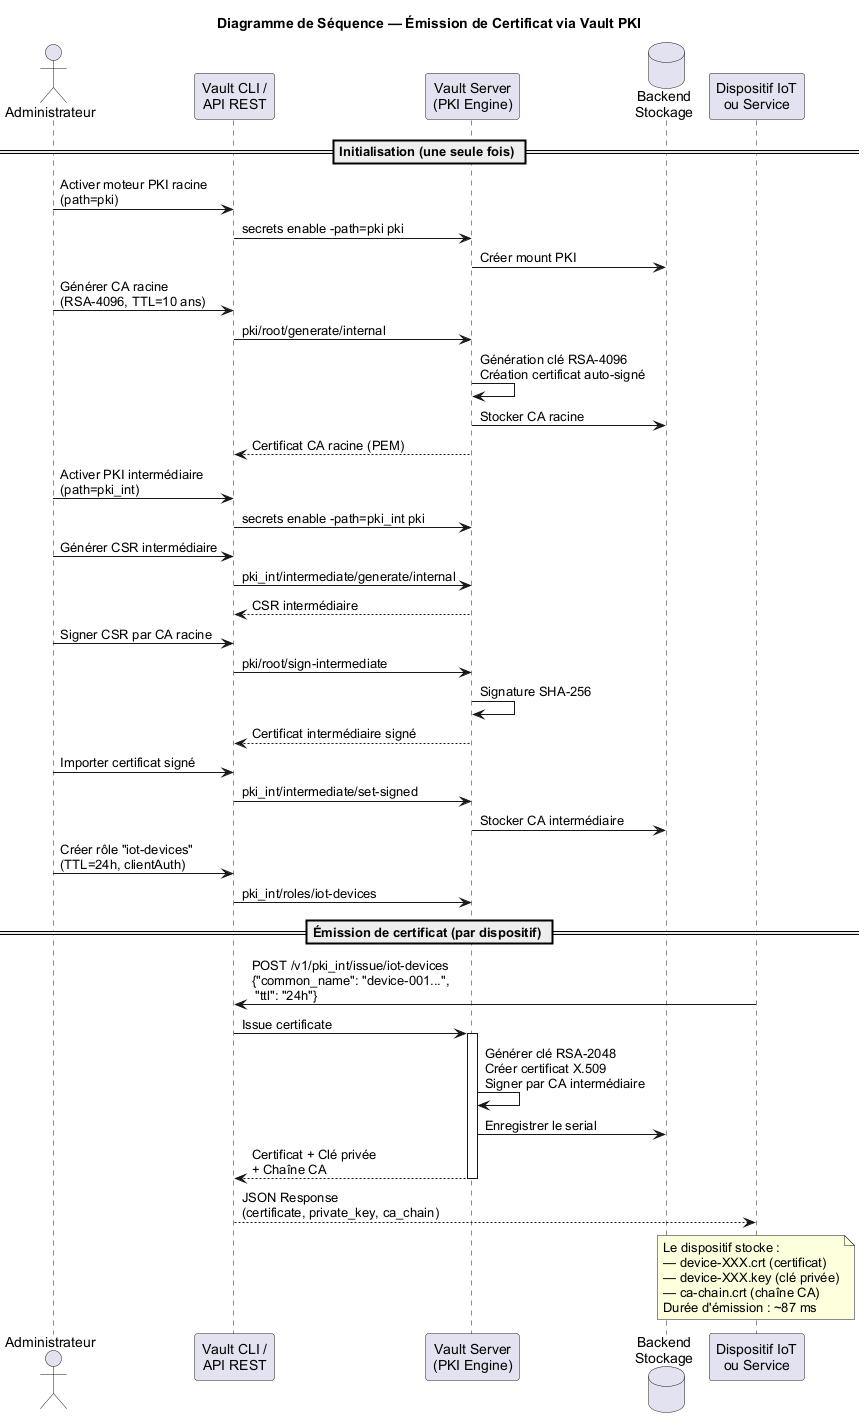
\includegraphics[width=0.85\textwidth]{diagrams/diag-pki-sequence.png}
  \caption{Séquence d'émission d'un certificat de dispositif via l'API Vault}
  \label{fig:pki_sequence}
\end{figure}

Pour chaque dispositif simulé, le script \texttt{generate\_device\_certs.sh} (Annexe~A, section~\ref{sec:script_gen_certs}) effectue un appel API REST au endpoint \texttt{/v1/pki\_int/issue/iot-devices} de Vault. La réponse contient :
\begin{itemize}
  \item Le certificat X.509 du dispositif.
  \item La clé privée associée.
  \item La chaîne de certification (CA intermédiaire + CA racine).
\end{itemize}

Ces éléments sont sauvegardés dans des fichiers PEM individuels, utilisés ensuite par le simulateur de flotte pour établir les connexions mTLS.

\section{Validation de la PKI}

La validité de la chaîne de certification est vérifiée à l'aide de l'outil \texttt{openssl verify}, qui confirme la chaîne : dispositif $\to$ CA intermédiaire $\to$ CA racine. Les commandes de validation sont détaillées en Annexe~A.

\begin{resultbox}[Résultat PKI]
\textbf{50 certificats de dispositifs} émis avec succès via l'API Vault. Chaîne de confiance validée : dispositif $\to$ CA intermédiaire $\to$ CA racine. Durée d'émission moyenne : \textbf{87~ms} par certificat via API REST.
\end{resultbox}
